\chapter{Background research and analysis}

\begin{landscape}
\section{Initial project Gantt chart}
\label{app:gantt1}
\begin{figure}[h!]
  \centering
   	\caption{Initial gantt chart, outline times throughout project activities, to be updated as time passes during the project span.}
      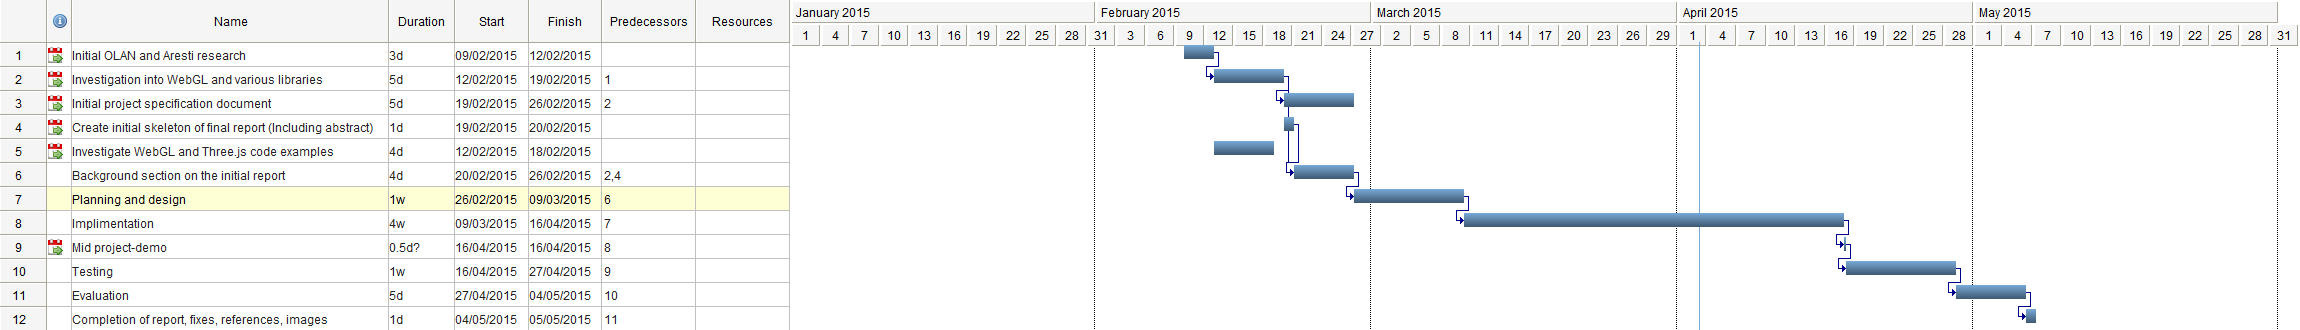
\includegraphics[width=23cm, height=6cm]{images/first.png}
\end{figure}
\end{landscape}
\clearpage

\section{Inital requirements analysis}
\label{app:init}
\begin{figure}[h!]
	\caption{Requirements brief created before a meeting to clarify questions on the initial requirements. The pdf continues onto the next page.}
	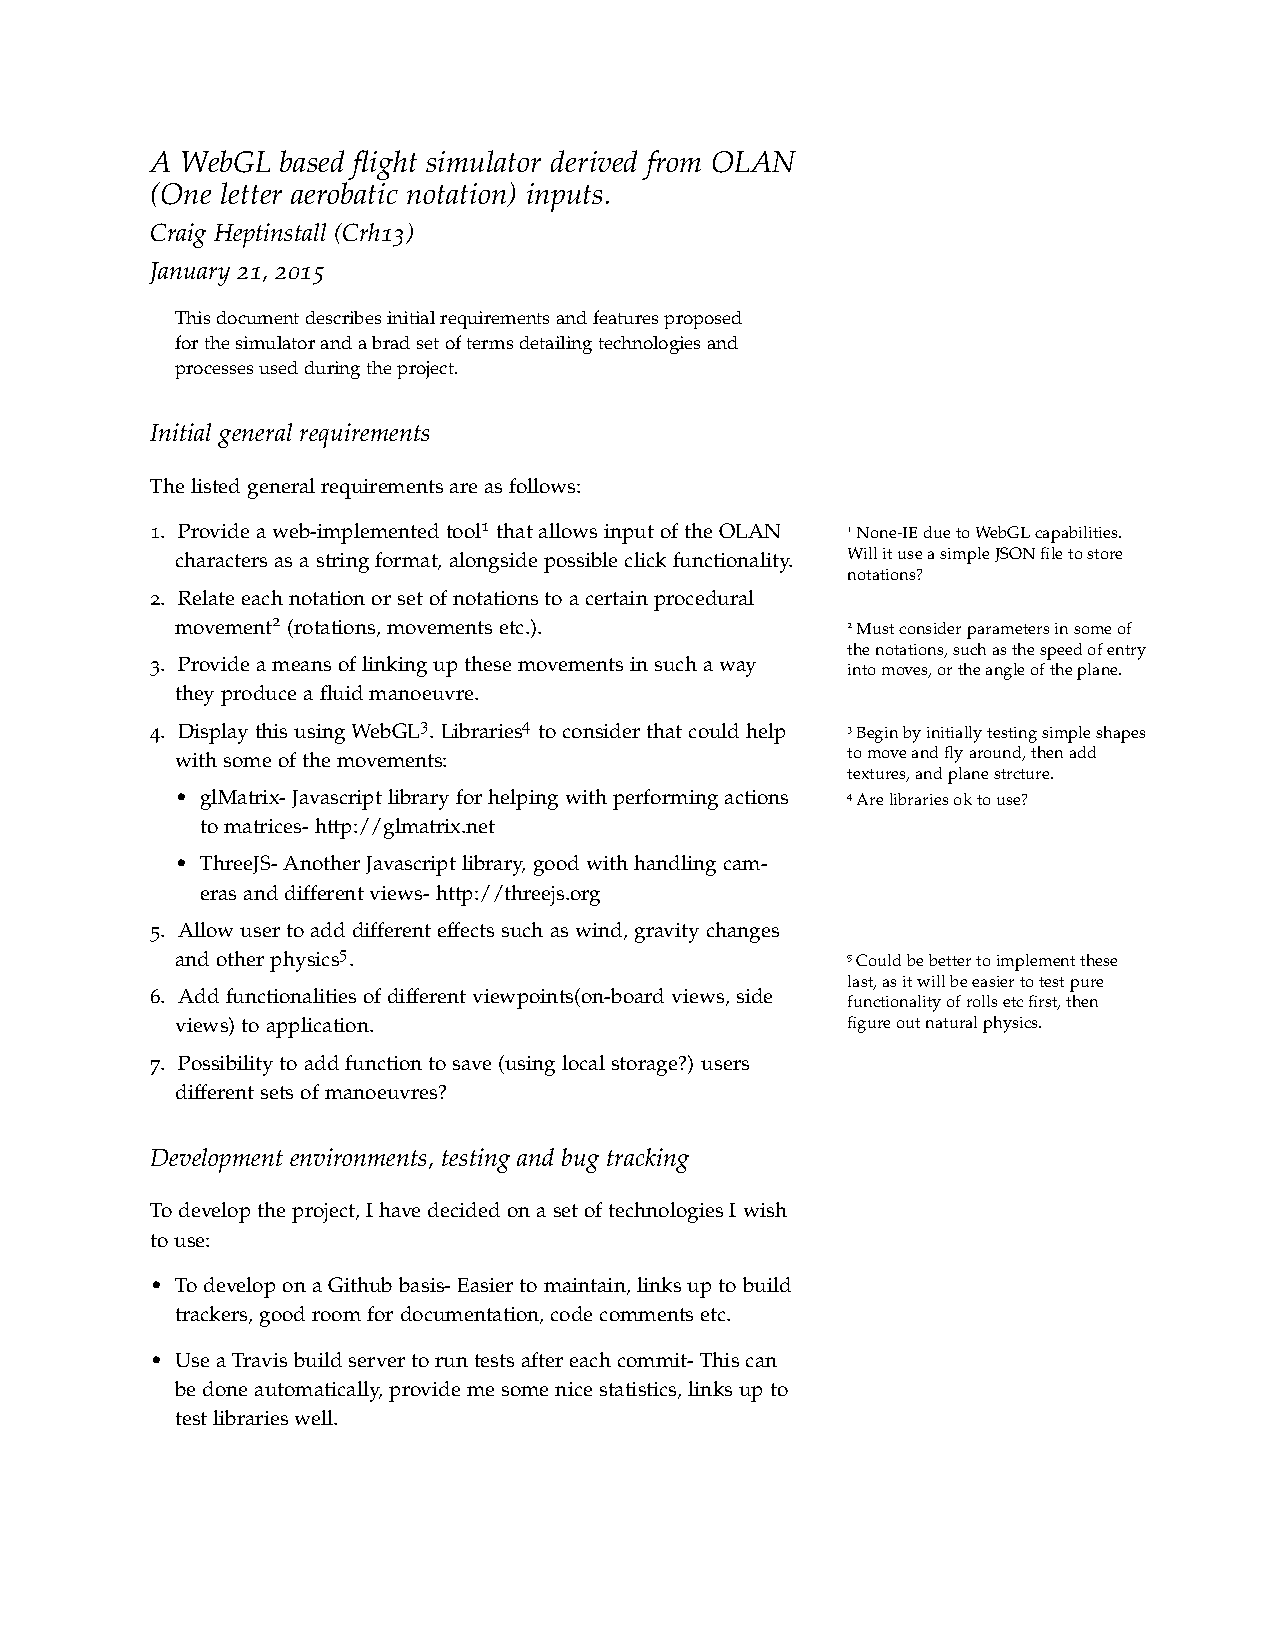
\includegraphics[width=18cm,height=18cm,page=1]{images/init.pdf}
\end{figure}

\begin{figure}[h!]
	\includegraphics[width=18cm,height=18cm,page=2]{images/init.pdf}
\end{figure}
\clearpage

\section{OLAN understandings}
\label{app:olan}
\begin{figure}[h!]
	\centering
	\caption{A document created before a second meeting, outlining my current undertsanding of the OLAN language, and how manoeuvres can be constructed from smaller single-element ones.}
	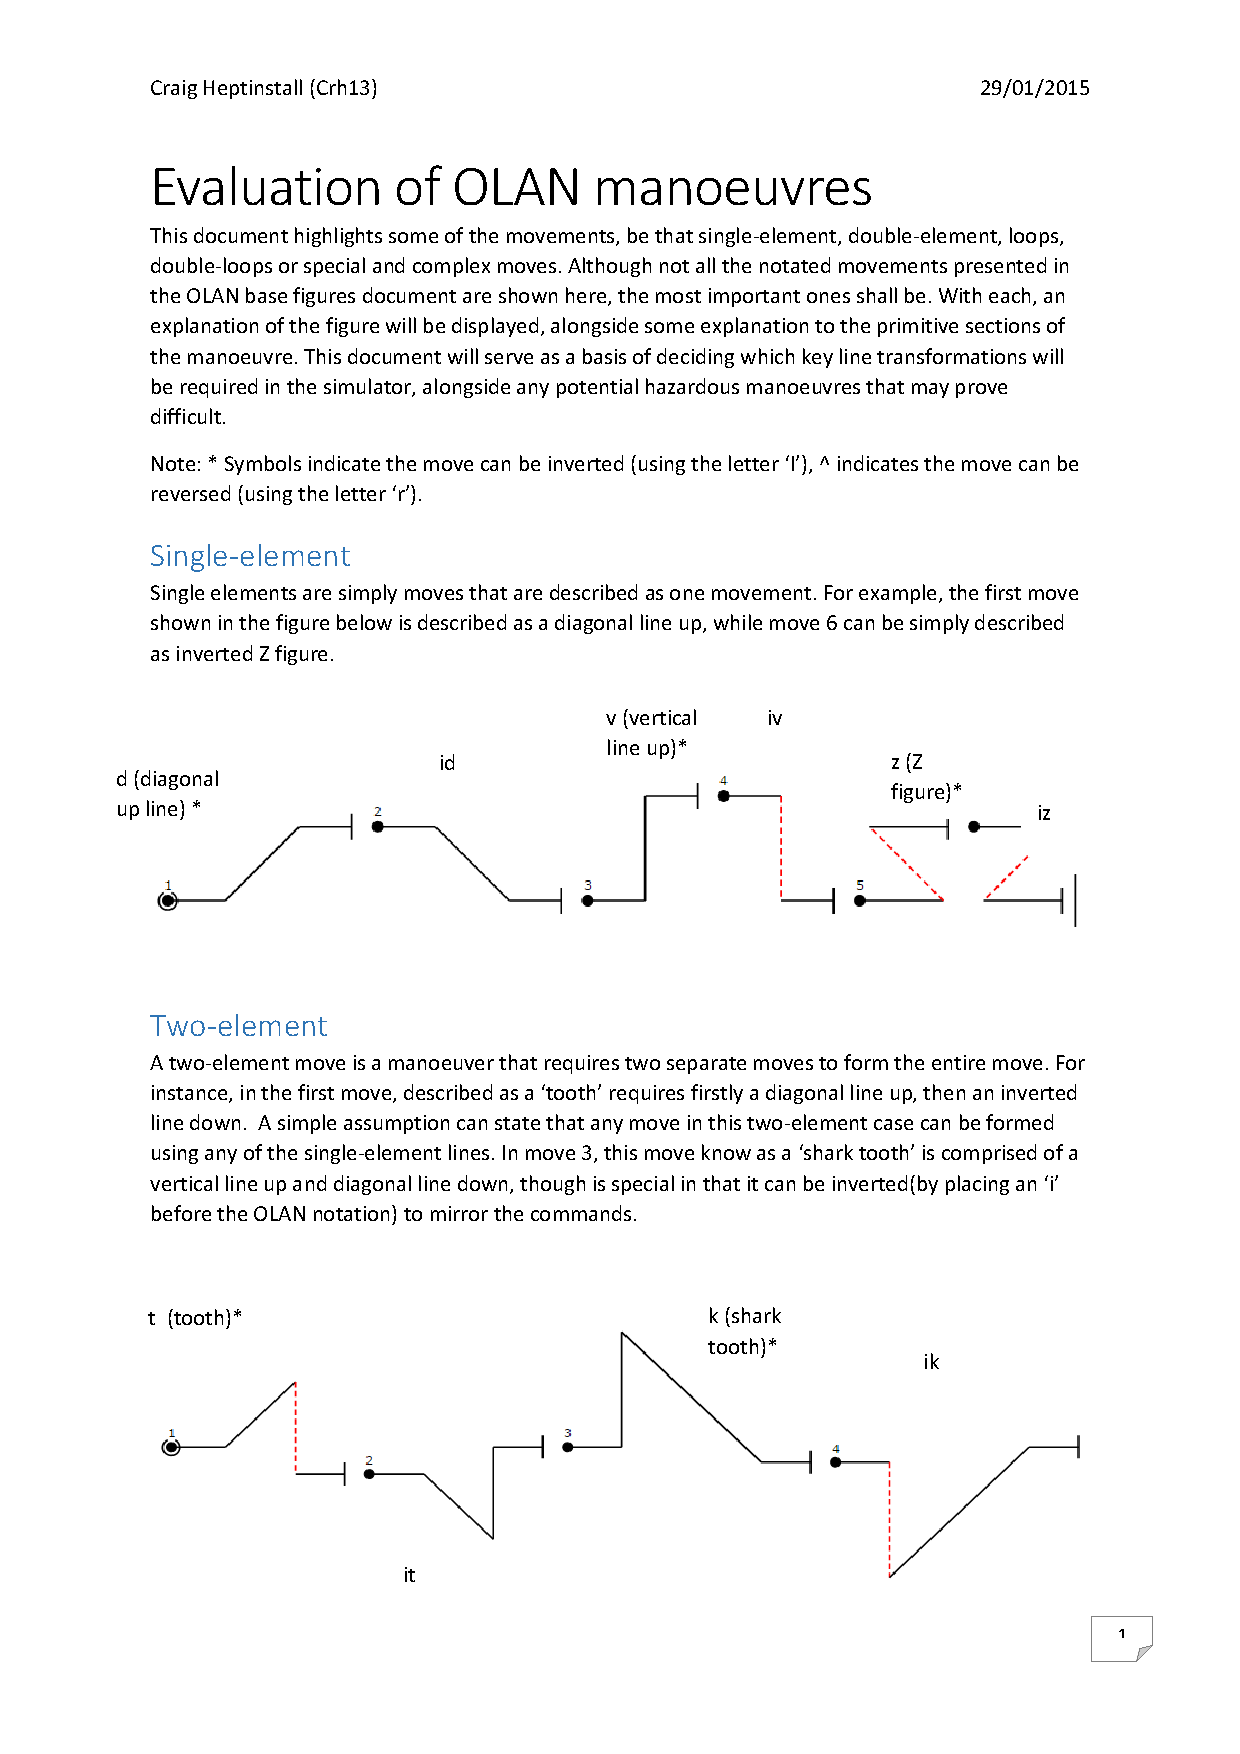
\includegraphics[width=16cm,height=20cm,page=1]{images/eval.pdf}
\end{figure}
\begin{figure}[h!]
	\centering
	\includegraphics[width=16cm,height=21cm,page=2]{images/eval.pdf}
\end{figure}
\begin{figure}[h!]
	\centering
	\includegraphics[width=16cm,height=21cm,page=3]{images/eval.pdf}
\end{figure}
\begin{figure}[h!]
	\centering
	\includegraphics[width=16cm,height=21cm,page=4]{images/eval.pdf}
\end{figure}
\begin{figure}[h!]
	\centering
	\includegraphics[width=16cm,height=21cm,page=5]{images/eval.pdf}
\end{figure}

\clearpage

\begin{landscape}
\section{Revised FDD Gantt chart}
\label{app:gantt2}
\begin{figure}[h!]
  \centering
  	\caption{More detailed Gantt chart, focuses on the implimentation and testing stratedgy of each feature. As you can see, prioritised tasks are the first to be completed.}
      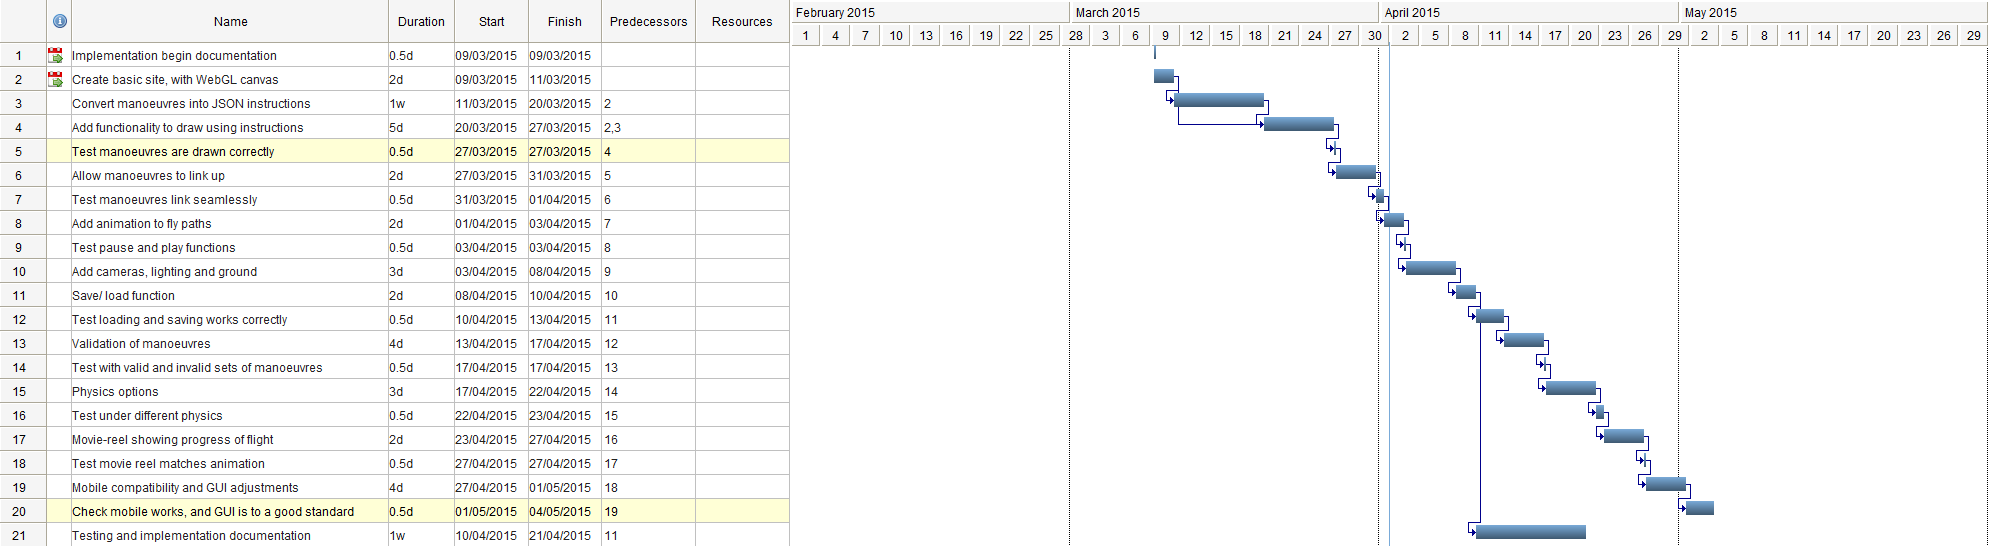
\includegraphics[width=23cm, height=6cm]{images/second.png}
\end{figure}
\end{landscape}
\clearpage